% move all configuration stuff into includes file so we can focus on the content
\documentclass[aspectratio=169,hyperref={pdfpagelabels=false,colorlinks=true,linkcolor=white,urlcolor=blue},t]{beamer}

%%%%%%%%%%%%%%%%%%%%%%%%%%%%%%%%%%%%%%%%%%%%%%%%%%%%%%%%%%%%%%%%%%%%%%%%%%%%%%%%%%
%%%%%%%%%%%%%%%%%%%%%%%%%%%%%%%%%%%%%%%%%%%%%%%%%%%%%%%%%%%%%%%%%%%%%%%%%%%%%%%%%%
% packages
\usepackage{pict2e}
\usepackage{epic}
\usepackage{amsmath,amsfonts,amssymb}
\usepackage{units}
\usepackage{fancybox}
\usepackage[absolute,overlay]{textpos} 
\usepackage{media9} % avi2flv: "C:\Program Files\ffmpeg\bin\ffmpeg.exe" -i TuneFreqFilterbank.avi -b 600k -s 441x324 -r 15 -acodec copy TuneFreqFilterbank.flv
\usepackage{animate}
\usepackage{gensymb}
\usepackage{multirow}
\usepackage{silence}
\usepackage{tikz}
\usepackage[backend=bibtex,style=ieee]{biblatex}
\AtEveryCitekey{\iffootnote{\tiny}{}}
\addbibresource{include/references}

%%%%%%%%%%%%%%%%%%%%%%%%%%%%%%%%%%%%%%%%%%%%%%%%%%%%%%%%%%%%%%%%%%%%%%%%%%%%%%%%%%
%%%%%%%%%%%%%%%%%%%%%%%%%%%%%%%%%%%%%%%%%%%%%%%%%%%%%%%%%%%%%%%%%%%%%%%%%%%%%%%%%%
% relative paths
\graphicspath{{graph/}}


%%%%%%%%%%%%%%%%%%%%%%%%%%%%%%%%%%%%%%%%%%%%%%%%%%%%%%%%%%%%%%%%%%%%%%%%%%%%%%%%%%
%%%%%%%%%%%%%%%%%%%%%%%%%%%%%%%%%%%%%%%%%%%%%%%%%%%%%%%%%%%%%%%%%%%%%%%%%%%%%%%%%%
% units
\setlength{\unitlength}{1mm}

%%%%%%%%%%%%%%%%%%%%%%%%%%%%%%%%%%%%%%%%%%%%%%%%%%%%%%%%%%%%%%%%%%%%%%%%%%%%%%%%%%
%%%%%%%%%%%%%%%%%%%%%%%%%%%%%%%%%%%%%%%%%%%%%%%%%%%%%%%%%%%%%%%%%%%%%%%%%%%%%%%%%%
% theme & layout
\usetheme{Frankfurt}
\beamertemplatenavigationsymbolsempty
%\setbeamertemplate{frametitle}[smoothbars theme]
\setbeamertemplate{frametitle}
{
    \begin{beamercolorbox}[ht=1.8em,wd=\paperwidth]{frametitle}
        \vspace{-.1em}%
        \hspace{.2em}{\strut\insertframetitle\strut}
        
        \hspace{.2em}\small\strut\insertframesubtitle\strut
        %\hfill
        %\includegraphics[height=.8cm,keepaspectratio]{CenterMusicTechnology-solid-2lines-white-CoAtag}
        
    \end{beamercolorbox}
    \begin{textblock*}{100mm}(11.6cm,.7cm)
        \includegraphics[height=.8cm,keepaspectratio]{Logo_GTCMT_black}
    \end{textblock*}
}
\setbeamertemplate{footline}[frame number]

% set this to ensure bulletpoints without subsections
\usepackage{remreset}
\makeatletter
\@removefromreset{subsection}{section}
\makeatother
\setcounter{subsection}{1}

%---------------------------------------------------------------------------------
% appearance
\setbeamercolor{structure}{fg=gtgold}
\setbeamercovered{transparent} %invisible
\setbeamercolor{bibliography entry author}{fg=black}
\setbeamercolor*{bibliography entry title}{fg=black}
\setbeamercolor*{bibliography entry note}{fg=black}
\setbeamercolor{frametitle}{fg=black}
\setbeamercolor{title}{fg=black}

%\usepackage{pgfpages}
%\setbeameroption{show notes}
%\setbeameroption{show notes on second screen=right}
%---------------------------------------------------------------------------------
% fontsize
\let\Tiny=\tiny

%%%%%%%%%%%%%%%%%%%%%%%%%%%%%%%%%%%%%%%%%%%%%%%%%%%%%%%%%%%%%%%%%%%%%%%%%%%%%%%%%%
%%%%%%%%%%%%%%%%%%%%%%%%%%%%%%%%%%%%%%%%%%%%%%%%%%%%%%%%%%%%%%%%%%%%%%%%%%%%%%%%%%
% warnings
\pdfsuppresswarningpagegroup=1
\WarningFilter{biblatex}{Patching footnotes failed}
\WarningFilter{latexfont}{Font shape}
\WarningFilter{latexfont}{Some font shapes}
\WarningFilter{gensymb}{Not defining}


%%%%%%%%%%%%%%%%%%%%%%%%%%%%%%%%%%%%%%%%%%%%%%%%%%%%%%%%%%%%%%%%%%%%%%%%%%%%%%%%%%
%%%%%%%%%%%%%%%%%%%%%%%%%%%%%%%%%%%%%%%%%%%%%%%%%%%%%%%%%%%%%%%%%%%%%%%%%%%%%%%%%%
% theme & layout
\usetheme{Frankfurt}
\useinnertheme{rectangles}


%%%%%%%%%%%%%%%%%%%%%%%%%%%%%%%%%%%%%%%%%%%%%%%%%%%%%%%%%%%%%%%%%%%%%%%%%%%%%%%%%%
\setbeamertemplate{frametitle}[default][colsep=-4bp,rounded=false,shadow=false]
\setbeamertemplate{frametitle}
{%
    \nointerlineskip%
    %\vskip-0.5ex
    \begin{beamercolorbox}[wd=\paperwidth,ht=3.5ex,dp=0.6ex]{frametitle}
        \hspace*{1.3ex}\insertframetitle%
        
        \hspace*{1.3ex}\small\insertframesubtitle%
    \end{beamercolorbox}%
    \begin{textblock*}{100mm}(11.6cm,.57cm)
        
\includegraphics[height=.8cm,keepaspectratio]{graph/Logo_GTCMT_white}
    \end{textblock*}
}


%%%%%%%%%%%%%%%%%%%%%%%%%%%%%%%%%%%%%%%%%%%%%%%%%%%%%%%%%%%%%%%%%%%%%%%%%%%%%%%%%%
\setbeamertemplate{title page}[default][colsep=-4bp,rounded=false,shadow=false]
\setbeamertemplate{title page}
{
    \begin{textblock*}{100mm}(15cm,.51cm)
            \href{https://github.com/alexanderlerch/ACA-Slides/blob/2nd_edition/\jobname.pdf}{\includegraphics[height=.5cm,keepaspectratio]{graph/Logo_github}}\hspace*{2ex}
    \end{textblock*}
    \vskip-10ex
    \begin{beamercolorbox}[wd=\paperwidth,ht=.7\paperheight,dp=0.6ex]{frametitle} %35ex
        %\begin{flushright}
            %\href{http://www.gtcmt.gatech.edu}{\includegraphics[height=.8cm,keepaspectratio]{graph/Logo_GTCMT_black}}\hspace*{2ex}
        %\end{flushright}
        
        \hspace*{1.8ex}\LARGE\inserttitle%
        
        \vspace*{.5ex}
        
        \hspace*{1.3ex}\small\insertsubtitle%
        
        \vspace*{.5ex}
    \end{beamercolorbox}%
    \nointerlineskip%
    \begin{beamercolorbox}[wd=\paperwidth,ht=.4\paperheight,dp=0.6ex]{page number in head/foot}
        %\vspace*{-.5ex}
        \hspace*{1.7ex}\small\insertauthor%
        
        %\hspace*{1.7ex}\small }%
        
        \vspace*{10ex}
        
        \begin{flushright}
            \href{http://www.gtcmt.gatech.edu}{\includegraphics[height=.8cm,keepaspectratio]{graph/Logo_GTCMT_black}}\hspace*{2ex}
        \end{flushright}
    \end{beamercolorbox}%
}


%%%%%%%%%%%%%%%%%%%%%%%%%%%%%%%%%%%%%%%%%%%%%%%%%%%%%%%%%%%%%%%%%%%%%%%%%%%%%%%%%%
%\makeatother
\setbeamertemplate{footline}
{
  \leavevmode%
  \hbox{%
  \begin{beamercolorbox}[wd=.5\paperwidth,ht=2.25ex,dp=1ex,left,leftskip=1ex]{page number in head/foot}%
    \insertsubtitle
  \end{beamercolorbox}%
  \begin{beamercolorbox}[wd=.5\paperwidth,ht=2.25ex,dp=1ex,right,rightskip=1ex]{page number in head/foot}%
    \hfill
    \insertframenumber{} / \inserttotalframenumber
  \end{beamercolorbox}}%
  \vskip0pt%
}
%\makeatletter


%%%%%%%%%%%%%%%%%%%%%%%%%%%%%%%%%%%%%%%%%%%%%%%%%%%%%%%%%%%%%%%%%%%%%%%%%%%%%%%%%%
\beamertemplatenavigationsymbolsempty
\setbeamertemplate{navigation symbols}{}
\setbeamertemplate{blocks}[default]%[rounded=false,shadow=false]
\setbeamertemplate{itemize item}[square]
\setbeamertemplate{itemize subitem}[circle]
\setbeamertemplate{itemize subsubitem}[triangle]
\setbeamertemplate{enumerate item}[square]
\setbeamertemplate{enumerate subitem}[circle]
\setbeamertemplate{enumerate subsubitem}[circle]


%%%%%%%%%%%%%%%%%%%%%%%%%%%%%%%%%%%%%%%%%%%%%%%%%%%%%%%%%%%%%%%%%%%%%%%%%%%%%%%%%%
% colors
\setbeamercolor{structure}{fg=darkgray}
\setbeamercovered{transparent} %invisible
\setbeamercolor{bibliography entry author}{fg=black}
\setbeamercolor*{bibliography entry title}{fg=black}
\setbeamercolor*{bibliography entry note}{fg=black}
\setbeamercolor{frametitle}{fg=black}
\setbeamercolor{title}{fg=white}
\setbeamercolor{subtitle}{fg=white}
\setbeamercolor{frametitle}{fg=white}
\setbeamercolor{framesubtitle}{fg=white}
\setbeamercolor{mini frame}{fg=white, bg=black}
\setbeamercolor{section in head/foot}{fg=white, bg=darkgray}
\setbeamercolor{page number in head/foot}{fg=black, bg=lightblue}
\setbeamercolor{item projected}{fg=white, bg=black}

%---------------------------------------------------------------------------------
%%%%%%%%%%%%%%%%%%%%%%%%%%%%%%%%%%%%%%%%%%%%%%%%%%%%%%%%%%%%%%%%%%%%%%%%%%%%%%%%%%
%%%%%%%%%%%%%%%%%%%%%%%%%%%%%%%%%%%%%%%%%%%%%%%%%%%%%%%%%%%%%%%%%%%%%%%%%%%%%%%%%%
% title information
\title[]{Introduction to \textbf{Audio Content Analysis}}   
\author[alexander lerch]{alexander lerch} 
%\institute{~}
%\date[Alexander Lerch]{}
%\titlegraphic{\vspace{-16mm}\includegraphics[width=\textwidth,height=3cm]{title}}

%%%%%%%%%%%%%%%%%%%%%%%%%%%%%%%%%%%%%%%%%%%%%%%%%%%%%%%%%%%%%%%%%%%%%%%%%%%%%%%%%%
%%%%%%%%%%%%%%%%%%%%%%%%%%%%%%%%%%%%%%%%%%%%%%%%%%%%%%%%%%%%%%%%%%%%%%%%%%%%%%%%%%
% colors
\definecolor{gtgold}{HTML}{E0AA0F} %{rgb}{0.88,0.66,1,0.06} [234, 170, 0]/256
\definecolor{darkgray}{rgb}{.1, .1, .25}
\definecolor{lightblue}{rgb}{.1, 0.75, 1}
\definecolor{highlight}{rgb}{0, 0, 1} %_less!40

%%%%%%%%%%%%%%%%%%%%%%%%%%%%%%%%%%%%%%%%%%%%%%%%%%%%%%%%%%%%%%%%%%%%%%%%%%%%%%%%%%
%%%%%%%%%%%%%%%%%%%%%%%%%%%%%%%%%%%%%%%%%%%%%%%%%%%%%%%%%%%%%%%%%%%%%%%%%%%%%%%%%%
% relative paths
\graphicspath{{../ACA-Plots/graph/}}


%%%%%%%%%%%%%%%%%%%%%%%%%%%%%%%%%%%%%%%%%%%%%%%%%%%%%%%%%%%%%%%%%%%%%%%%%%%%%%%%%%
%%%%%%%%%%%%%%%%%%%%%%%%%%%%%%%%%%%%%%%%%%%%%%%%%%%%%%%%%%%%%%%%%%%%%%%%%%%%%%%%%%
% units
\setlength{\unitlength}{1mm}

%%%%%%%%%%%%%%%%%%%%%%%%%%%%%%%%%%%%%%%%%%%%%%%%%%%%%%%%%%%%%%%%%%%%%%%%%%%%%%%%%%
%%%%%%%%%%%%%%%%%%%%%%%%%%%%%%%%%%%%%%%%%%%%%%%%%%%%%%%%%%%%%%%%%%%%%%%%%%%%%%%%%%
% math
\DeclareMathOperator*{\argmax}{argmax}
\DeclareMathOperator*{\argmin}{argmin}
\DeclareMathOperator*{\atan}{atan}
\DeclareMathOperator*{\arcsinh}{arcsinh}
\DeclareMathOperator*{\sign}{sign}
\DeclareMathOperator*{\tcdf}{tcdf}
\DeclareMathOperator*{\si}{sinc}
\DeclareMathOperator*{\princarg}{princarg}
\DeclareMathOperator*{\arccosh}{arccosh}
\DeclareMathOperator*{\hwr}{HWR}
\DeclareMathOperator*{\flip}{flip}
\DeclareMathOperator*{\sinc}{sinc}
\DeclareMathOperator*{\floor}{floor}
\newcommand{\e}{{e}}
\newcommand{\jom}{\mathrm{j}\omega}
\newcommand{\jOm}{\mathrm{j}\Omega}
\newcommand   {\mat}[1]    		{\boldsymbol{\uppercase{#1}}}		%bold
\renewcommand {\vec}[1]    		{\boldsymbol{\lowercase{#1}}}		%bold

%%%%%%%%%%%%%%%%%%%%%%%%%%%%%%%%%%%%%%%%%%%%%%%%%%%%%%%%%%%%%%%%%%%%%%%%%%%%%%%%%%
%%%%%%%%%%%%%%%%%%%%%%%%%%%%%%%%%%%%%%%%%%%%%%%%%%%%%%%%%%%%%%%%%%%%%%%%%%%%%%%%%%
% media9
\newcommand{\includeaudio}[1]{
\href{run:audio/#1.mp3}{
\includegraphics[width=5mm, height=5mm]{graph/SpeakerIcon}}}

\newcommand{\includeanimation}[4]{{\begin{center}
                        \animategraphics[autoplay,loop,scale=.7]{#4}{animation/#1-}{#2}{#3}        
                        \end{center}
                        \addreference{matlab source: \href{https://github.com/alexanderlerch/ACA-Plots/blob/master/matlab/animate#1.m}{matlab/animate#1.m}}}
                        \inserticon{video}}
                        
%%%%%%%%%%%%%%%%%%%%%%%%%%%%%%%%%%%%%%%%%%%%%%%%%%%%%%%%%%%%%%%%%%%%%%%%%%%%%%%%%%
%%%%%%%%%%%%%%%%%%%%%%%%%%%%%%%%%%%%%%%%%%%%%%%%%%%%%%%%%%%%%%%%%%%%%%%%%%%%%%%%%%
% other commands
\newcommand{\question}[1]{%\vspace{-4mm}
                          \setbeamercovered{invisible}
                          \begin{columns}[T]
                            \column{.9\textwidth}
                                \textbf{#1}
                            \column{.1\textwidth}
                                \vspace{-8mm}
                                \begin{flushright}
                                     
\includegraphics[width=.9\columnwidth]{graph/question_mark}
                                \end{flushright}
                                \vspace{6mm}
                          \end{columns}\pause\vspace{-12mm}}

\newcommand{\toremember}[1]{
                        \inserticon{lightbulb}
                        }

\newcommand{\matlabexercise}[1]{%\vspace{-4mm}
                          \setbeamercovered{invisible}
                          \begin{columns}[T]
                            \column{.8\textwidth}
                                \textbf{matlab exercise}: #1
                            \column{.2\textwidth}
                                \begin{flushright}
                                     \includegraphics[scale=.5]{graph/logo_matlab}
                                \end{flushright}
                                %\vspace{6mm}
                          \end{columns}}

\newcommand{\addreference}[1]{  
                  
                    \begin{textblock*}{\baselineskip }(.98\paperwidth,.5\textheight) %(1.15\textwidth,.4\textheight)
                         \begin{minipage}[b][.5\paperheight][b]{1cm}%
                            \vfill%
                             \rotatebox{90}{\tiny {#1}}
                        \end{minipage}
                   \end{textblock*}
                    }
                    
\newcommand{\figwithmatlab}[1]{
                    \begin{figure}
                        \centering
                        \includegraphics[scale=.7]{#1}
                        %\label{fig:#1}
                    \end{figure}
                    
                    \addreference{matlab source: \href{https://github.com/alexanderlerch/ACA-Plots/blob/main/matlab/plot#1.m}{plot#1.m}}}
\newcommand{\figwithref}[2]{
                    \begin{figure}
                        \centering
                        \includegraphics[scale=.7]{#1}
                        \label{fig:#1}
                    \end{figure}
                    
                    \addreference{#2}}  
                                    
\newcommand{\inserticon}[1]{
                    \begin{textblock*}{100mm}(14.5cm,7.5cm)
                        \includegraphics[height=.8cm,keepaspectratio]{graph/#1}
                    \end{textblock*}}            

%%%%%%%%%%%%%%%%%%%%%%%%%%%%%%%%%%%%%%%%%%%%%%%%%%%%%%%%%%%%%%%%%%%%%%%%%%%%%%%%%%
%%%%%%%%%%%%%%%%%%%%%%%%%%%%%%%%%%%%%%%%%%%%%%%%%%%%%%%%%%%%%%%%%%%%%%%%%%%%%%%%%%
% counters
\newcounter{i}
\newcounter{j}
\newcounter{iXOffset}
\newcounter{iYOffset}
\newcounter{iXBlockSize}
\newcounter{iYBlockSize}
\newcounter{iYBlockSizeDiv2}
\newcounter{iXBlockSizeDiv2}
\newcounter{iDistance}




\subtitle{module B.6: frequency resolution \& instantaneous frequency}

%%%%%%%%%%%%%%%%%%%%%%%%%%%%%%%%%%%%%%%%%%%%%%%%%%%%%%%%%%%%%%%%%%%%%%%%%%%%
\begin{document}
    % generate title page
	{
\setbeamertemplate{headline}{} 
\setbeamertemplate{footline}{} 
\begin{frame}
    \titlepage
    %\vspace{-5mm}
\end{frame}
}
\addtocounter{framenumber}{-1}


    \section[overview]{lecture overview}
        \begin{frame}{introduction}{overview}
            \begin{block}{corresponding textbook section}
                \begin{itemize}
                    %\item \href{http://ieeexplore.ieee.org/xpl/articleDetails.jsp?tp=&arnumber=6331119&}{Chapter 2~---~Fundamentals}: pp.~21--23
                    %\item   \href{http://ieeexplore.ieee.org/xpl/articleDetails.jsp?arnumber=6331122}{Chapter 5~---~Tonal Analysis}: pp.~92--93
                    \item section~7.3.1
                    \item appendix~B.6
                \end{itemize}
            \end{block}

            \begin{itemize}
                \item   \textbf{lecture content}
                    \begin{itemize}
                        \item   frequency detection error for sampled signals
                        \item   instantaneous frequency/frequency reassignment
                    \end{itemize}
                \bigskip
                \item<2->   \textbf{learning objectives}
                    \begin{itemize}
                        \item   list the factors influencing frequency resolution in time and frequency domains
                        \item   explain the frequency error in Cent
                        \item   implement an instantaneous frequency estimate
                    \end{itemize}
            \end{itemize}
            \inserticon{directions}
        \end{frame}

    \section[intro]{introduction}
        \begin{frame}{pitch detection resolution}{introduction}
            \begin{itemize}
                \item (fundamental) frequency detection on digital signals (discrete in time and frequency)
                \item[$\Rightarrow$] quantized result
            \end{itemize}
            
            \pause
            
            error being made due to \textit{discrete} signal processing
            
            \begin{itemize}
                \item   \textbf{time domain}:
                    \begin{itemize}
                        \item   detection of \textit{period length}
                        \item[$\Rightarrow$] maximum error depends on distance between two samples (sample rate)
                    \end{itemize}
                \bigskip
                \item<3->   \textbf{frequency domain}:
                    \begin{itemize}
                        \item detection of \textit{bin frequency}
                        \item[$\Rightarrow$] maximum error depends on distance between two frequency bins (block length and sample rate)
                    \end{itemize}
                %\bigskip
                %\item<4->[] \textbf{BUT}
                    %\begin{itemize}
                        %\item<5->   a more meaningful error metric is neither \unit{s} nor \unit{Hz} but \textit{Cent}
                    %\end{itemize}
            \end{itemize}
        \end{frame}
        \begin{frame}{pitch detection resolution}{time domain (e.g., ACF)}
            \vspace{-2mm}
            period length quantized to multiple of inter-sample interval $T_\mathrm{S}$
            \begin{eqnarray*}
                &T_\mathrm{Q} &= j\cdot T_{\mathrm{S}}\\
                \Rightarrow &f_\mathrm{Q} &= \frac{1}{j\cdot T_{\mathrm{S}}}
            \end{eqnarray*}
            \vspace{-5mm}
            \figwithmatlab{PitchErrorTimeDomain}
        \end{frame}
        \begin{frame}{pitch detection resolution}{frequency domain (e.g., HPS)}
		frequency quantized to multiple of inter-bin interval
		 \begin{equation*}
		 	f_\mathrm{Q} = k\cdot\frac{f_{\mathrm{S}}}{\mathcal{K}} 
		 \end{equation*}
		 \only<1>
		 {
			\begin{footnotesize}\begin{table}
				\centering
				\begin{tabular}{lccc} %{c|p{12mm}p{12mm}p{12mm}p{12mm}p{12mm}p{12mm}p{12mm}}
                    \\ \hline
                    \bf{\emph{$\mathcal{K}$}}	 & \bf{\emph{$\Delta f\;[\unit{Hz}]$}}	 & \bf{\emph{$k_\mathrm{ST}$}}	 & \bf{\emph{$f(k_\mathrm{ST})\;[\unit{Hz}]$}}\\ 
                     \hline
                    \bf{256}	 & 187.5	 & 35	 & 6562.5\\
                    \bf{512}	 & 93.75	 & 35	 & 3281.25\\
                    \bf{1024}	 & 46.875	 & 35	 & 1640.625\\
                    \bf{2048}	 & 23.4375	 & 35	 & 820.3125\\
                    \bf{4096}	 & 11.7188	 & 35	 & 410.1563\\
                    \bf{8192}	 & 5.8594	 & 35	 & 205.0781\\
                    \bf{16384}	 & 2.9297	 & 35	 & 102.5391\\
				\end{tabular}
			\end{table}\end{footnotesize}
		}
		\only<2>
		{
            \vspace{-3mm}
            \figwithmatlab{PitchErrorFreqDomain}
        }
        \end{frame}
    \section[solutions]{improving the frequency resolution}
        \begin{frame}{pitch detection resolution}{simple fix}
            \begin{itemize}
                \item   \textbf{assumption}: pitch is stationary with minor deviations over time
                \bigskip
                \item<2-> \textbf{simple solution}: 
                    \begin{itemize}
                        \item   average pitch observations over blocks
                        \item   the more blocks are averaged, the more result might approximate the \textit{real} (population) mean
                    \end{itemize}
                \bigskip
                \item<3->   \textbf{problems}:
                    \begin{enumerate}
                        \item   adds significant latency (non-realtime)
                        \item   will not work for time-variant signals (speech, music)
                    \end{enumerate}
            \end{itemize}
        \end{frame}
    
        \begin{frame}{pitch detection resolution}{time domain observations}
            \figwithmatlab{PitchErrorTimeDomain}
            
            \begin{itemize}
                \item   error depends on fundamental frequency
                \item   error depends on sample rate
            \end{itemize}
        \end{frame}
        \begin{frame}{pitch detection resolution}{time domain workarounds}
            \vspace{-2mm}
            virtually increase time resolution by upsampling
            \figwithmatlab{TimeInterp}
            
            \begin{enumerate}
                \item[$+$] higher virtual resolution
                \item[$-$] significant workload increase
            \end{enumerate}
        \end{frame}
	
    %\section[frequency domain]{improving the pitch tracking resolution}
        \begin{frame}{pitch detection resolution}{frequency domain workarounds}
            different ways of increasing frequency resolution in the frequency domain
            \begin{enumerate}
                \item<1->   increasing the FFT window length (decreases time resolution)
                \bigskip
                \item<2->   interpolating  the spectrum
                \bigskip
                \item<3->   applying frequency reassignment
            \end{enumerate}
        \end{frame}

        \begin{frame}{pitch detection resolution}{spectrum interpolation}
            \begin{columns}
            \column {.4\linewidth}
            \begin{enumerate}
                \item<1->   zeropad in time domain
                \bigskip
                \bigskip
                \bigskip
                \item<1->   use standard interpolation on magnitude spectrum
            \end{enumerate}
            \column {.6\linewidth}
                \figwithmatlab{FreqInterp}%
            \end{columns}
            %\addreference{matlab source: \href{https://github.com/alexanderlerch/ACA-Slides/blob/master/matlab/displayFreqResolution.m}{matlab/displayFreqResolution.m}}
        \end{frame}
    \section{frequency reassignment}
        \begin{frame}{pitch detection resolution}{frequency reassignment: relation of phase and frequency 1/2}
            \begin{columns}
            \column{.5\linewidth}
            \vspace{-10mm}
            \includeanimation
                {Phasor}
                {00}
                {160}
                {10}
            %\begin{center}
                %\animategraphics[autoplay,loop]{10}{animatePhasor/Phasor-}{00}{80}        
            %\end{center}
            \column{.5\linewidth}
           \begin{itemize}
                \item   phasor representation:
                    \begin{enumerate}
                        \item   sine value is defined by magnitude and phase
                        \item   decreasing the amplitude $\Rightarrow$ shorter vector
                        \item   increasing the frequency $\Rightarrow$ increasing speed
                    \end{enumerate}
            \end{itemize}
            \end{columns}
                        %\addreference{matlab source: \href{https://github.com/alexanderlerch/ACA-Slides/blob/master/matlab/animatePhasor.m}{matlab/animatePhasor.m}}
            \inserticon{video}

        \end{frame}
        \begin{frame}{pitch detection resolution}{frequency reassignment: relation of phase and frequency 2/2}

            \begin{columns}
            \column{0.3\textwidth}
                \begin{figure}
                \begin{tiny}
                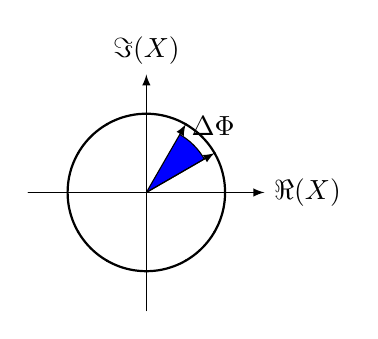
\begin{tikzpicture}[scale=1,cap=round,>=latex]
                    % draw the coordinates
                    \draw[->] (-1.5cm,0cm) -- (1.5cm,0cm) node[right,fill=white] {$\Re(X)$};
                    \draw[->] (0cm,-1.5cm) -- (0cm,1.5cm) node[above,fill=white] {$\Im(X)$};
        
                    \draw[fill=highlight] (0,0) -- (30:.85cm) arc (30:60:.85cm);
                    \draw (45:1.2cm) node {$\Delta\Phi$};
                    \draw[->] (0cm,0cm) -- (0.8660cm,0.5cm);
                    \draw[->] (0cm,0cm) -- (0.5cm,0.8660cm);
        
                    % draw the unit circle
                    \draw[thick] (0cm,0cm) circle(1cm);
            
                    \foreach \x in {0,30,...,360} {
        %	                % dots at each point
                            \filldraw[black] (\x:1cm) circle(0.2pt);
                    }
                \end{tikzpicture}
                \end{tiny}
                \end{figure}
             \column{0.7\textwidth}
            \begin{itemize}
                \item   relation of frequency and phase change:
                    \begin{itemize}
                        \item<2-> time for full rotation is period length $T$ with \[f = \frac{1}{T}\]
                        \item<3-> time for fractional rotation $\Delta\Phi$ is corresponding fraction of period length \[f = \frac{\Delta\Phi}{\Delta t}\]
                        \item<4-> in other words: 
                        \begin{eqnarray*}
                            \Phi(t) &=& \omega\cdot t\\
                            \Rightarrow \frac{d\Phi(t)}{dt} &=& \omega = 2\pi f
                        \end{eqnarray*}
                    \end{itemize}
            \end{itemize}
            \end{columns}
        \end{frame}
        \begin{frame}{pitch detection resolution}{frequency reassignment: principles}
            frequency domain:
            \begin{itemize}
                \item   instead of using the bin frequency
                    \[ f(k) = k\cdot\frac{f_\mathrm{S}}{\mathcal{K}}\]
                \item   we use the phase of each bin $\Phi(k,n)$
                \item   to compute the frequency from the phase difference of neighboring blocks
                    \begin{equation*}\label{eq:phasediff}
                        \omega_{\mathrm{I}}(k,n)	\propto \Phi(k,n)-\Phi(k,n-1)
                    \end{equation*}
                \item<2->   $\omega_{\mathrm{I}}(k,n)$ is called \textbf{instantaneous frequency} per block per bin
            \end{itemize}
        \end{frame}
        \begin{frame}{pitch detection resolution}{frequency reassignment: scaling factor}
            \begin{itemize}
                \item instantaneous frequency calculation has to take into account
                    \begin{itemize}
                        \item   hop size $\mathcal{H}$
                        \item   sample rate $f_\mathrm{S}$
                    \end{itemize}
                
                    \begin{equation*}
                        \omega_{\mathrm{I}}(k,n) = \frac{\Delta\Phi_{\mathrm{u}}(k,n)}{\mathcal{H}}\cdot f_{\mathrm{S}} 
                    \end{equation*}
                \item<1-> problem: phase ambiguity
                    \begin{equation*}
                        \Phi(k,n) = \Phi(k,n) + j\cdot 2\pi
                    \end{equation*}
                \item<2->[$\Rightarrow$] \textit{phase unwrapping}
            \end{itemize}
        \end{frame}
        \begin{frame}{pitch detection resolution}{frequency reassignment: phase unwrapping}

            \begin{enumerate}
                \item	compute unwrapped phase $\Phi_{\mathrm{u}}(k,n)$ 
                        \begin{itemize}
                            \item	estimate unwrapped bin phase
                                    \begin{footnotesize}
                                    \begin{equation*}\label{eq:phi_est}
                                        \hat{\Phi}(k,n) = \Phi(k,n-1) + \underbrace{2\pi k\cdot\frac{\mathcal{H}}{\mathcal{K}}}_{=\omega_k\cdot\frac{\mathcal{H}}{f_\mathrm{s}}} 
                                    \end{equation*}
                                    \end{footnotesize}

                            \item<2->	unwrap phase by shifting current phase to estimate's range
                                    \begin{footnotesize}
                                    \begin{equation*}
                                        \Phi_{\mathrm{u}}(k,n) = \hat{\Phi}(k,n) + \princarg\left[ \Phi(k,n) - \hat{\Phi}(k,n) \right]
                                    \end{equation*}
                                    \end{footnotesize}
                        \end{itemize}

                \item<3->	compute unwrapped phase difference
                        \begin{footnotesize}
                        \begin{eqnarray*}
                            \Delta\Phi_{\mathrm{u}}(k,n)	&=& \Phi_{\mathrm{u}}(k,n) - \Phi(k,n-1)\nonumber\\
                                                \pause
                                                &=& \hat{\Phi}(k,n) + \princarg\left[ \Phi(k,n) - \hat{\Phi}(k,n) \right] - \Phi(k,n-1)\nonumber \\
                                                \pause
                                                &=& \frac{2\pi k}{\mathcal{K}}\mathcal{H} + \princarg\left[ \Phi(k,n) - \Phi(k,n-1) - \frac{2\pi k}{\mathcal{K}}\mathcal{H} \right]\nonumber
                        \end{eqnarray*}
                        \end{footnotesize}
            \end{enumerate}
        
        \end{frame}
        \begin{frame}{pitch detection resolution}{frequency reassignment: problems}
                \begin{itemize}
                    \item   \textbf{overlapping spectral components}
                        \begin{itemize}
                            \item   sinusoidal components often overlap (spectral leakage, several instruments playing the same pitch, ...)
                                \begin{itemize}
                                    \item[$\Rightarrow$] ``incorrect'' phase estimate
                                    \item<1-> spectrum should be as sparse as possible, increase STFT length
                                \end{itemize}
                        \end{itemize}
                    \bigskip
                    \item<2->   \textbf{inaccurate phase unwrapping} 
                        \begin{itemize}
                            \item   unwrapping algorithm is based on assumption of similarity between predicted and measured phase
                            \item<2-> decrease hop size
                        \end{itemize}
                \end{itemize}
        \end{frame}
        \begin{frame}{pitch detection resolution}{frequency reassignment: example}
            \figwithmatlab{InstantaneousFreq}
            \begin{columns}
            \column{.5\linewidth}
            \begin{itemize}
                \item   FFT length: 1024
                \item   sample rate: \unit[48]{kHz}
            \end{itemize}
            \column{.5\linewidth}
            \begin{itemize}
                \item   selected frequencies: 
                    \begin{itemize}
                        \item   between bins (0.5)
                        \item   between bins (0.25)
                        \item   on bin
                    \end{itemize}
            \end{itemize}
            \end{columns}
        \end{frame}

            
        \begin{frame}{pitch detection resolution}{frequency reassignment: applications}
            \begin{itemize}
                \item \textbf{improving frequency resolution}
                    \begin{itemize}
                        \item e.g., for detecting signal frequencies when using a filter bank
                    \end{itemize}
                \bigskip
                \item<2-> \textbf{improving phase extrapolation}
                    \begin{itemize}
                        \item e.g., for accurate phase estimation in the \textit{phase vocoder}
                    \end{itemize}
                \bigskip
                \item<3-> \textbf{grouping spectral bins}
                    \begin{itemize}
                        \item spectral leakage sidelobes have the same instantaneous frequency
                    \end{itemize}
                \bigskip
                \item<4-> \textbf{tonalness detection}
                    \begin{itemize}
                        \item   the instantaneous frequency should be reasonably close to the bin frequency for the component to be considered tonal
                    \end{itemize}
            \end{itemize}
        \end{frame}
        
   \section[summary]{summary}
        \begin{frame}{summary}{lecture content}
            \begin{itemize}
                \item   \textbf{frequency resolution of sampled signals depends on}
                    \begin{itemize}
                        \item   time domain: sample rate
                        \item   freq domain: sample rate, block size
                    \end{itemize}
                \bigskip
                \item   \textbf{pitch detection error \textsl{in Cent} also depends on input frequency}
                    \begin{itemize}
                        \item   time domain: high error at high frequencies
                        \item   freq domain: high error at low frequencies
                    \end{itemize}
                \bigskip
                \item   \textbf{possible solutions}
                    \begin{itemize}
                        \item   time domain: 
                            \begin{itemize}
                                \item upsampling/interpolation
                            \end{itemize}
                        \item   freq domain: 
                            \begin{itemize}
                                \item   zeropadding/interpolation
                                \item   frequency reassignment (instantaneous frequency)
                            \end{itemize}
                    \end{itemize}
            \end{itemize}
            \inserticon{summary}
        \end{frame}
\end{document}
